\documentclass[11pt]{article}
\usepackage[utf8]{inputenc}

\usepackage{amssymb}
\usepackage{amsmath}
\usepackage{amsthm}
\usepackage{graphicx} 
\usepackage{fullpage}
\usepackage[ruled,vlined,linesnumbered]{algorithm2e}
\usepackage{wrapfig}

\setlength{\parindent}{0em}  % set the indent of the paragraph
\setlength{\parskip}{0em} % set the space of the paragraph

\theoremstyle{definition}
\newtheorem{definition}{Definition}[section] % add the section number in front of the definition number
% \newtheorem*{definition}{Definition} % remove the index number of the definition

\title{Data	Exploration Project}
\author{Xianlin Feng}
\date{\today}

\begin{document}
\maketitle

\section{Introduction}
\label{Introduction}
Road traffic accident is a threat to all people in their daily life. According to the WHO's statistics in 2018, road traffic accidents are the eighth of the top 10 causes of death, which is the only reason of injuries, and all the remaining reason are diseases. In the worldwide, road injuries took 140 million lives in 2016, in which $74\%$ are were men and boys. (https://www.who.int/news-room/fact-sheets/detail/the-top-10-causes-of-death). Serious situation happened in Victoria too. There were 58 lives lost because of the road accident every day in 2018 just in Victoria. This number increased to 88 since 7 April 2019. In the last five years, the least worse situation happened in 2017, the daily lives lost was 64.  According to the TAC report, the lives lost of drivers takes nearly half ($48.2\%$) of the daily lives lost. The age of death is concentrated in 30-69 years old. The most lives lost in rural roads($58\%$).(http://www.tac.vic.gov.au/road-safety/statistics/lives-lost-year-to-date). The analysis of past traffic accidents can provide a basis for future road construction, accident prevention, and accident rescue. The following three question will be answered in this report:
\begin{enumerate}
	\item What is the trend in the last 13 years?
	\item What is the main cause of road crashes in Victoria.
	\item What suggestion we can provide for the people in different areas.
\end{enumerate}
To answer those three questions, I will try to analysis and explore the dataset to find the main cause of road crashes in Victoria, as well as the trend in the last 13 years. I will try to find one or more datasets, then perform data wrangling, data cleaning and data checking before data exploration. During the data exploration, I will perform different statistic tests and visualisation to explore the data set and obtain insight from the data. At last, I will provide some suggestions base on the result of the data exploration. The main structure of this report is as follow: the data wrangling will be processed in section \ref{dataWrangling}, then the data will be checking in section \ref{dataChecking}. The data exploration will be carried out in section \ref{dataExploration}, followed by the section of conclusion. In the last section, there will be a reflection of this assessment. 
\par


\section{Data Wrangling} 
\label{dataWrangling}
Usually the data we get is messy, incomplete or unformatted, which cannot be used for data analysis directly. Data wrangling is a process to manipulate data to make the data directly usable for analysis. According to "2016 Data Science Salary Survey",  data scientists spend 53\% of their time for data cleaning and data wrangling. (https://learning.oreilly.com/library/view/2016-data-science/9781492049029/). After data wrangling, the raw data is transformed into the data that can be analysed to generate insights and valid results. Data wrangling is vital for data science project, which not only improves the efficiency of data analysis, but also reduces the error caused by erroneous data. In this section, I will divide the data wrangling process into the following small tasks base on the characteristics of the data set:
\begin{enumerate}
	\item Introduce the data set
	\item Filter the data
	\item Time series data handling	
	\item Drop missing or null values in the dataset
	\item Grouping Data
	\item convert free text dates to standard format
	\item deal with outliers or "illegal" values
	\item discrete the data into a set of values
	\item data checking
\end{enumerate}


\subsection{the Dataset}
The data set I found for this project named "CrashStats data", which could be downloaded on Victoria government open data website: https://www.data.vic.gov.au . The dataset was provide by VicRoad for educational purposes, and it includes the crash data of time, location, conditions and so on since 2000. The dataset is consist with 12 tables in the following list:
\begin{enumerate}
	\item \textbf{accident}:	contain the besic information about the accident, such as date, time, location, environment codition and severity.
	\item \textbf{vehicle}:	vehicle information, such as make, body type, year of manufacture, fuel type, vechicle capacity and so on.
	\item \textbf{person}:	person details, such as age, sex, sitting position, passengers or driver, license state etc.	
	\item \textbf{accident$\_$event}: the sequence of events during the accident, such as ran off carriageway, collision, fell from vehicle, and so on.
	\item \textbf{accident$\_$location}:	the location information of the accident.
	\item \textbf{road$\_$surface$\_$cond}:	the codition of the road: wet, dry, or icy.
	\item \textbf{atmospheric$\_$cond}:	weather condition: clear, wind, dust and so on.
	\item \textbf{sub$\_$dca}:	describing the crash detail with code.
	\item \textbf{accident$\_$node}:	more detailed location about the crash.
	\item \textbf{accident$\_$chainage}:	chainage information of the node.
	\item \textbf{node$\_$id$\_$complex$\_$int$\_$id}:	if the node locate in a complex intersection or not.
	\item \textbf{statistic$\_$checks}:	the statistic information of the crashes in this dataset.
\end{enumerate}
Before the data wrangling and data cleaning, we need to understand the characteristics of each data table, for example, in the table of "accident", each accident has exact one record. But, as one accident may involved two or more people, one accident may have two or more records in the table "person". Same situation happens in table "vehicle", "accident$\_$event" and other tables too, this is another reason why this dataset separate to 12 data tables. Due to this reason, when we process data wrangling, data cleaning, or data exploration, extra careful should be paid with the multiple records for one accident. 

\subsection{Time series data handling}
In the original data set, the time information is stored in the format \text{"\textbf{hh.mm.ss}"}, which is not the common time format, so that I change them to the format \text{"\textbf{hh:mm:ss}"} first. This step could easily perform in Microsoft Excel by just replacing every "." by ":". Then, the date and time information are separated into two columns, which is not very friendly to Tableau Public, so we need to combine them together first. In order to complete this task, I need to insert a new column "\textbf{date$\&$time}" and in the cell "D2" use a Excel formulation \text{"\textbf{TEXT(B2,"d\/mm\/yyyy")\&" "\&TEXT(C2,"hh:mm:ss"})"}. This formulation could combine the date information in cell "B2" and time information in cell "C2" without lose any information. By applying this formulation to all rows, The new column could contain both date and time information could be generated.

\subsection{Filter data}	
The data of 2019 will not considered in this report, so that, before we perform any data checking and data analysis, they need to be filtered. In the table "ACCIDENT", this step could easily done in Tableau Public, since we have generated the new column named "\text{$\&$time}", we can just drag the field "date$\&$time" to the "filter", then select "year" and unselected "2019" for before any date analysis. For the other tables, as the date information is only stored in the "ACCIDENT" table, this action could be more complicate, but every record in other tables contains "accident$\_$ID" field. So that, a left outer join is essential for each table and table "ACCIDENT". 

\subsection{Identify key attributes}
\label{IdentifyKeyAttributes}
Another important step after selecting data is identify key attributes. Each data instance contains lots of information related to the accident, however some of them are not related to our project. So that, select the useful data and information will help us for data checking and data analysis. This step is performed in Tableau Public too. The list blow indicate the key attributes for each table, then data checking and correcting will be performed for each attribute:
\begin{enumerate}
	\item \textbf{accident}: accident number, date, time, type, day of week, accident type, light condition, node, involved vehicles, road condition and so on.
	\item \textbf{person}: sex, age, injured level, seating position, role, license information, movement. 
	\item \textbf{vehicle}: register state, make, model, year of manufacture, type, body style, number of person, color, level of damage, collision position. 
	\item \textbf{accident$\_$node}:	node$\_$ID, type, latitude, longitude. postcode.  
	\item \textbf{road$\_$surface$\_$cond}: road surface condition.
	\item \textbf{accident$\_$event}: event sequence, event type, collision position and so on.
	\item \textbf{accident$\_$location}:	 node$\_$ID, type of intersecting road, distance to the nearest intersecting road. 
	\item \textbf{atmospheric$\_$cond}:	atmospheric condition.
\end{enumerate}

\subsection{(Draft)Join tables}
\label{JoinTable}
Because of the different characteristics of each table, it hard to join two tables into one table. But there still some work can be done. For example, If we perform a left outer join the table "accident" and the table "accident$\_$node", base on the "node ID", we could get the geographic information for each accident. This could be easily done in Tableau Public. We could also perform the left outer join between the table "accident" and  the table "road$\_$surface$\_$cond" base on "accident$\_$ID", table "accident" and the table "accident$\_$location" as well as "atmospheric$\_$cond" base on "node$\_$ID". The structure of the joins is showing below:
\begin{figure}[h!]
	\begin{center}
		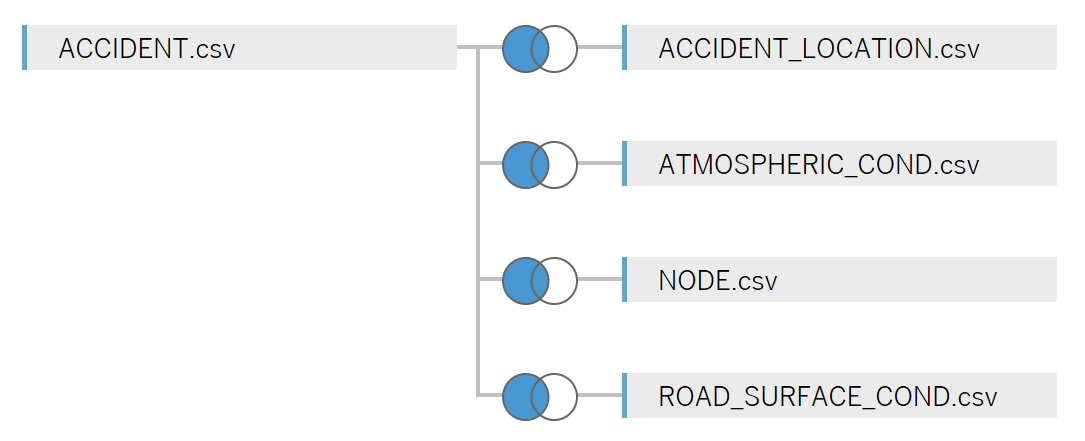
\includegraphics[scale=0.8]{images/leftouterjoin.png} 
	\end{center}
 	\label{fig:leftOuterJoin}
\caption{left outer joint structure}
\end{figure}


\section{Data Checking}
\label{dataChecking}
Tableau Public is a powerful tool for data wrangling, as well as data checking. In this section I will demonstrate the main step I performed for data checking. More specific, checking the key attributes of each table base on the property of the attribute. \\

\subsection{Check geographic data}
In the table "NODE", the attributes "lat" and "long" indicate the latitude and longitude coordinates for each accident. the attribute "Postcode$\_$No" demonstrate the suburb information. To check the attributes of "lat", "long" and "Postcode", just put them in the Tableau Public map, the result shows no record is outside Victoria state. so we can consider the geographic data is complete and consist.\par

\{draft\} And the attribute "NODE$\_$ID" is the index of the location for the accident. For the attribute of "NODE$\_ID$", we should check and remove the missing value and outlier, for example the "-3", "-10", as the negative number 

\subsection{Check duplicate record}
Eliminate duplicate records is important for data analysis. To complete this task, I used Tableau Public to identify the duplicate records in the key attributes. For example, for the "ACCIDENT$\_$No" in the table "ACCIDENT". The following command will calculate the time of one record appearance in the field. 
\begin{center}
\text{\{fixed[Accident$\_$No:SUM([Number of Records])\}}
\end{center}
The result shows there is no duplicate records in "ACCIDENT$\_$No" attributes.

\subsection{Check the missing value}
\begin{wrapfigure}{r}{0.5\textwidth}
	\vspace{-35pt}
	\begin{center}
	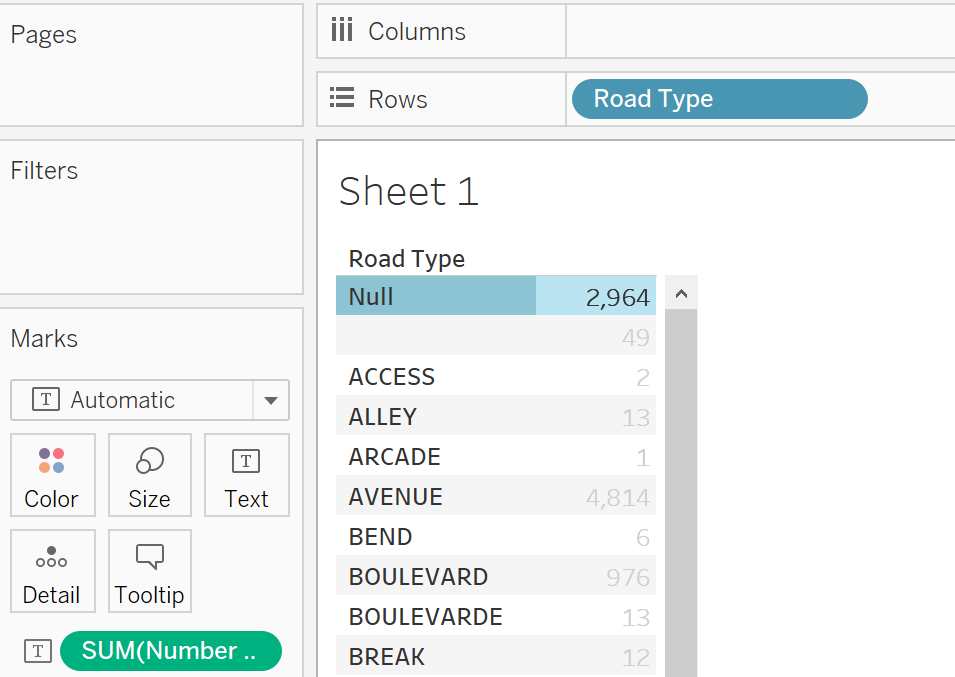
\includegraphics[width=0.9\linewidth]{images/IdentifyMissingValue.png}
	\end{center}
	\caption{Identify missing value}
	\vspace{-0pt}
\label{fig:identifyMissingValue}
\end{wrapfigure}	
In Tableau Public, we can identify the missing value by summarise the table or each filed. The picture on the right shows the missing value of attribute "Road Type" in table "ACCIDENT$\_$LOCATION". As it showing in figure \ref{fig:identifyMissingValue}, there are 2964 missing value for attribute "Road Type", but the missing values are not critical for the data analysis, so that I just ignore them.\par
Another method to deal with missing value is replacing the missing value with another value, such as 0. this could be done with function \textit{ZN()}, which could replacing any null value in the field with 0. 

\subsection{Check outlier}
To check outlier in the field, we should identify the range first. For example, when check the data range of the attribute "Node$\_$ID" in both table "ACCIDENT" and table "NODE" in Tableau Public, Two range could be found: $[4,\,342850]$ and $[-10,\,342850]$. Then I check the meta-data on the website of VicRoads. For the attribute of "Node$\_$ID", it explains that "The node id of the accident. It starts with 1 and incremented by one when a new accident location is indentified" % http://data.vicroads.vic.gov.au/metadata/Crash%20Stats%20-%20Data%20Extract%20-%20Open%20Data.html})
Therefore, the values blew 1 in the table "ACCIDENT" are outliers, and should not be used for analysis and exploration. Since the correct node id information is not known, the node id information cannot be used for analysing. Fortunately, the table "NODE" contains both accident information and node id information, and it will be used in the further data exploration.

\section{Data Exploration}
\label{dataExploration}
After data wrangling, cleaning, and checking, we have a clean and well formed data set to analysis. In this section, I will perform data exploration and data analysis mainly with Tableau Public. To answer the three questions proposed in section \ref{Introduction}, different statistics method and visualisation method will be used. I won't analysis all the attributes in the data set, but only the key attributes which is identified in the previous section.
\subsection{Trend of road crashes}
\begin{wrapfigure}{r}{0.5\textwidth}
	\vspace{-20pt}
	\begin{center}
	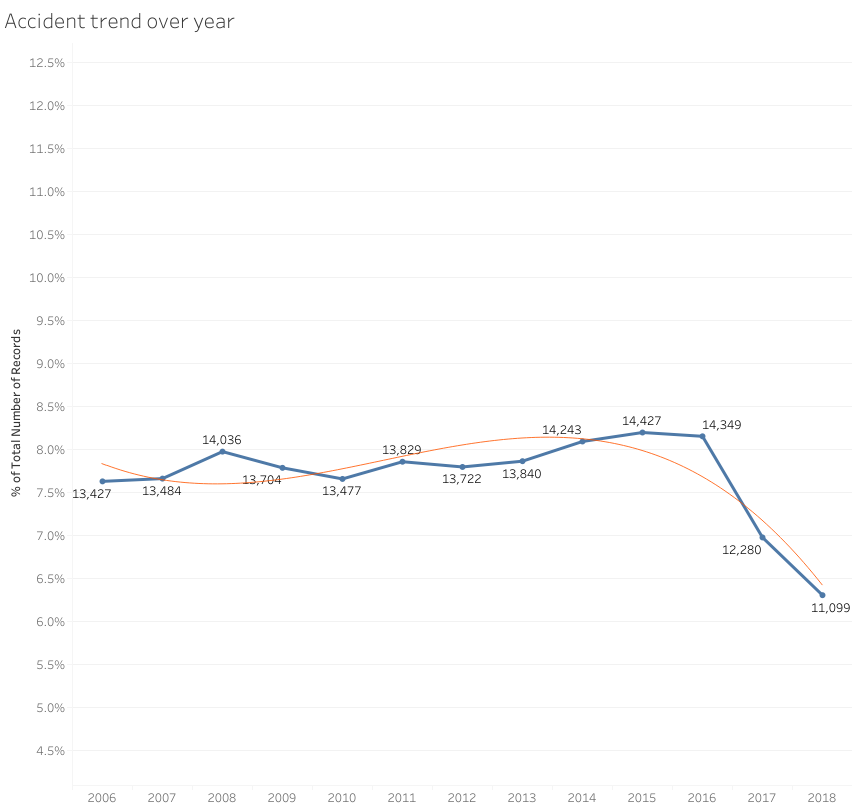
\includegraphics[width=0.9\linewidth]{images/trend_year.png}
	\end{center}
	\caption{Trend over the 13 years}
	\vspace{-0pt}
\label{fig:Trend over 13 years}
\end{wrapfigure}	
To answer this question, we need summarise each data table to identify the changes over 13 years. 



\subsection{main cause of road crashes in Victoria}
To identify the main cause 

\section{Conclusion}

\section{Reflection}





\end{document}
